\documentclass{article}

\usepackage{geometry}
\usepackage{makecell}
\usepackage{array}
\usepackage{multicol}
\usepackage{setspace}
\usepackage{changepage}
\usepackage{booktabs}
\usepackage{graphicx}
\usepackage{float}
\newcolumntype{?}{!{\vrule width 1pt}}
\renewcommand\theadalign{tl}
\setstretch{1.10}
\setlength{\parindent}{0pt}

\geometry{top=12mm, left=1cm, right=2cm}
\title{\vspace{-3cm}21S 520.230 Deutsch: Mutter-/Bildungssprache: Textanalyse und Textproduktion Gruppe 3}
\author{Andreas Hofer}

\begin{document}
	\begin{multicols}{2}
	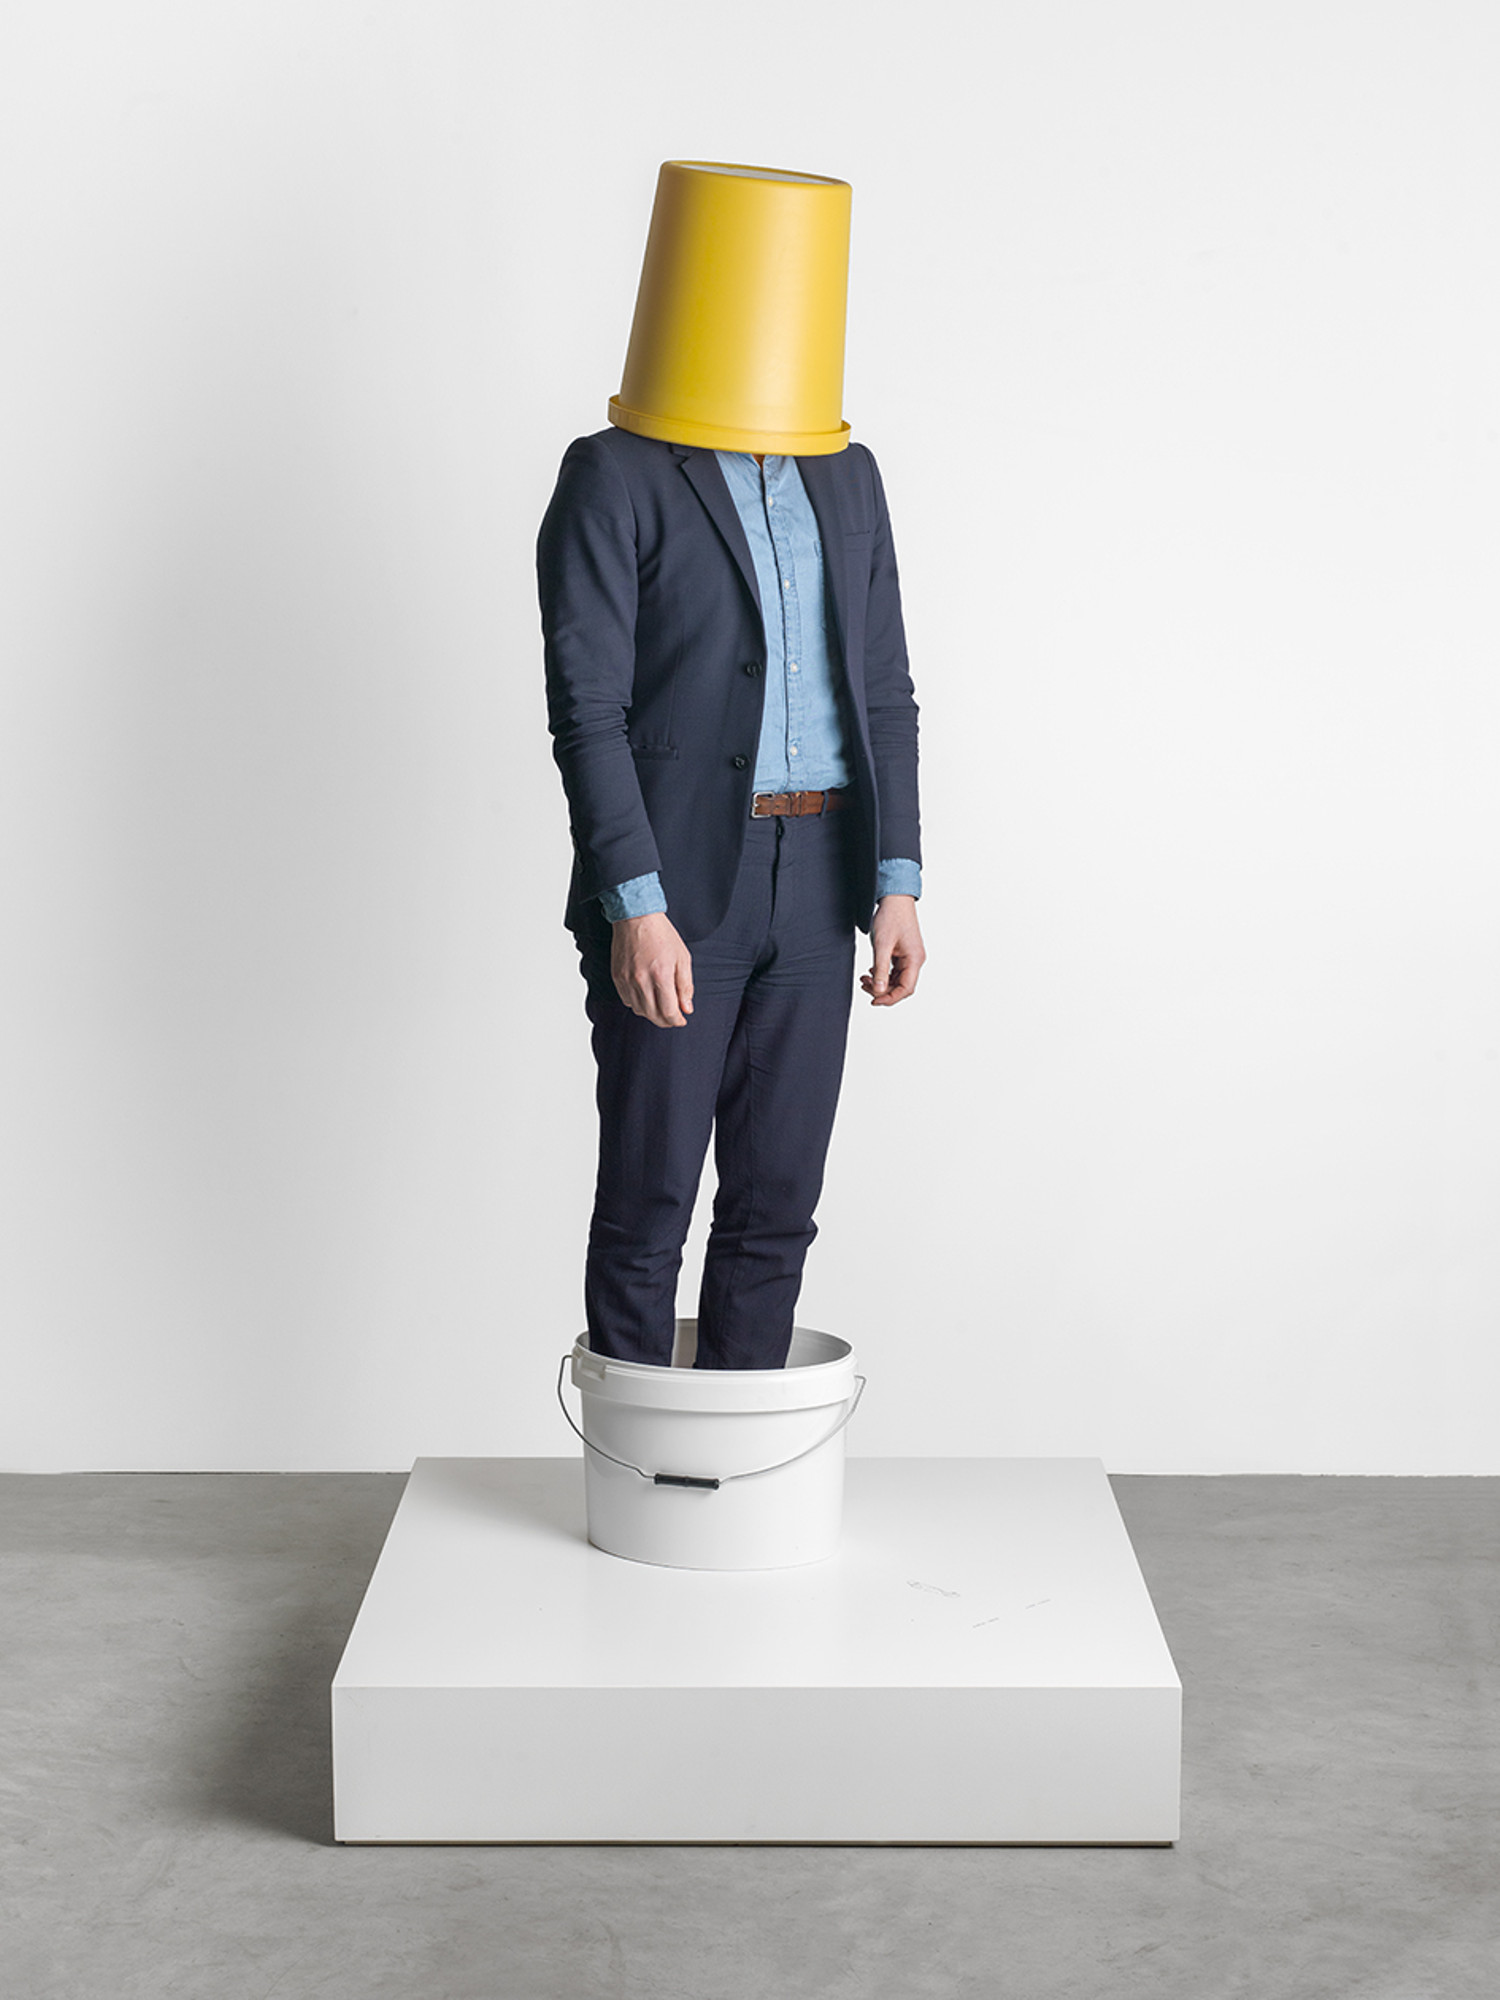
\includegraphics[width=90mm, height=100mm]{Eimer.jpg} \\
	\subsection*{Erwin Wurm: Statuen gesucht!}
	Man sagt ja immer, dass Kunst öde und vor Allem nur zum Anschauen ist. Erwin Wurm hat das offensichtlich überhört, denn bei ihm bist \textit{du} die Kunst. Ja, das hast du richtig gehört: Nicht nur dastehen und begutachten, sondern \textit{erleben}. Falls du dich also schon immer mit einem Eimer auf dem Kopf auf einem Podest präsentieren, und statt peinlichen Fragen wie "Was macht denn die da?", anerkennende Blicke ernten wolltest, dann schau rein ins Kunsthaus Graz. Erwin Wurm's Ausstellung "One-Minute-Statues" läuft dort nämlich von 16. März bis inklusive 31. April. Jugendlichen unter 16 Jahren winkt zusätzlich eine Ermäßigung von 50\%. \\ \\
	Kunsthaus Graz \\
	Lendkai 1, 8020 Graz \\
	T +43-316/8017-9200 \\
	info@kunsthausgraz.at \\ \\
	\textbf{Öffnungszeiten} \\
	Di-So, Feiertag 10 - 18 Uhr \\

	\columnbreak
	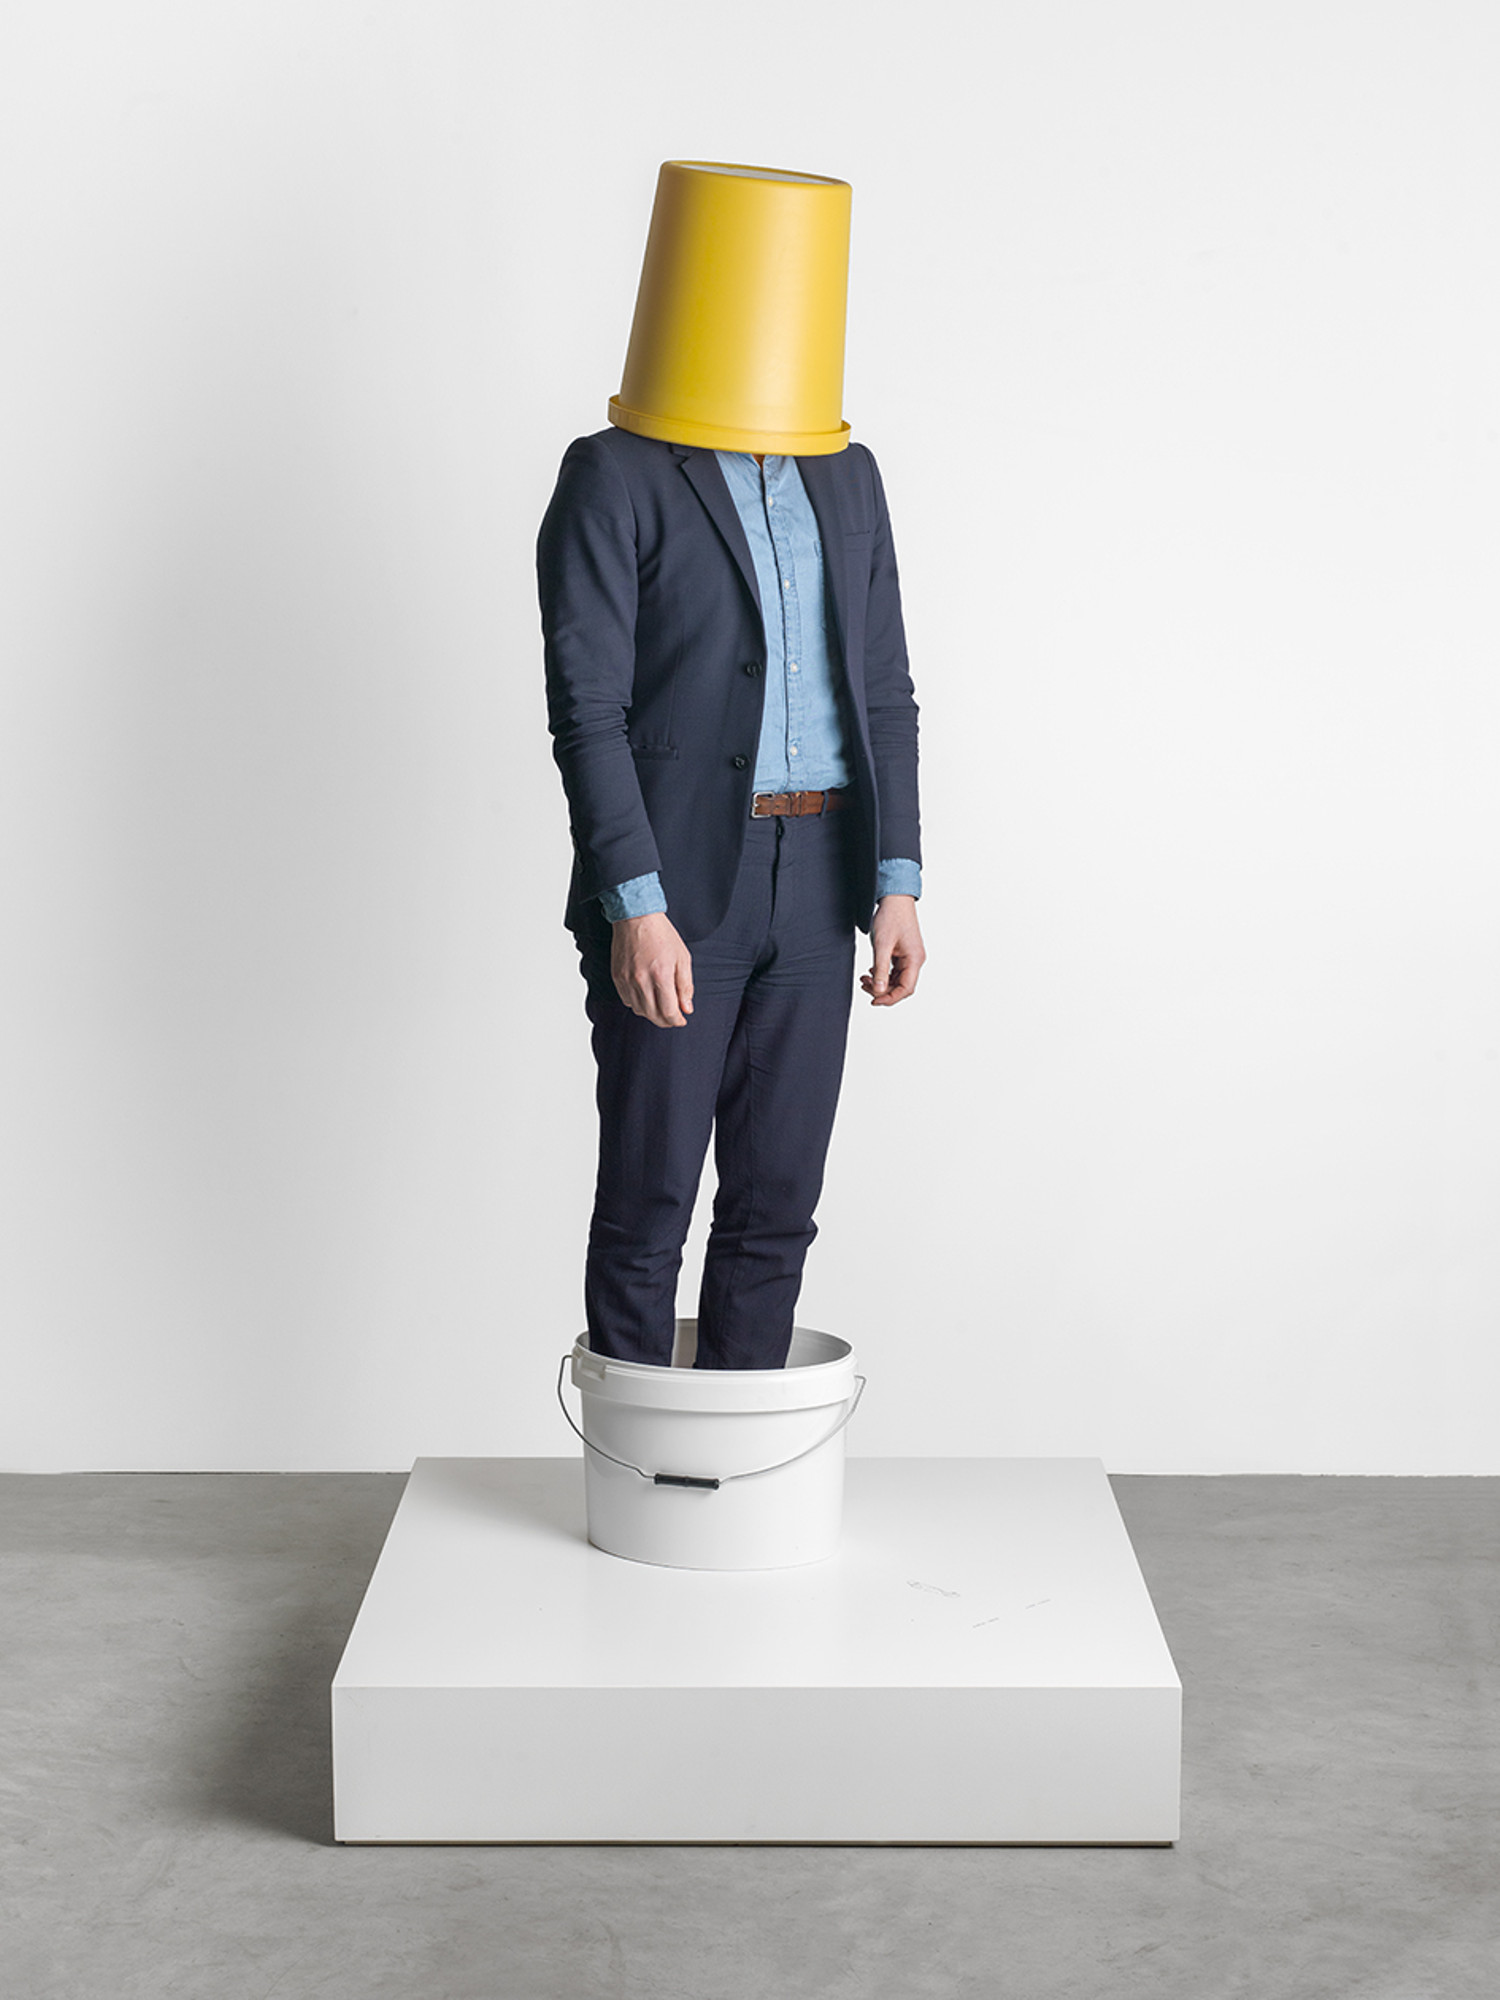
\includegraphics[width=90mm, height=100mm]{Eimer.jpg} \\
	\subsection*{Von fetten Häusern und kurzlebigen Skulpturen}
	Erwin Wurm ist nun seit einigen Jahren fester Bestandteil der österreichischen Kulturlandschaft. Nach erfolgreichen Ausstellungen in Wien und Salzburg, wo man unter anderem das "Fat House" im Belvedere sehen kann, ist er nun auch in Graz angekommen. Bekannt für seinen unorthodoxen Stil, macht er Besucher und Besucherinnen zu seinen Kunstobjekten indem er nur Requisiten und eine Anleitung zur Verfügung stellt. Tauchen Sie ein in eine Welt, in welcher die Grenzen zwischen Kunstobjekt und Beobachter zu verschwimmen scheinen. Und auch falls Sie selbst kein Interesse daran haben, bieten sich umfangreiche Sitzmöglichkeiten an, um das Kunstschaffen anderer mitverfolgen zu können. Bestaunen können Sie diese Entstehung der Skulpturen zwischen 16. März und 31. April im Kunsthaus Graz.\\ \\
	Kunsthaus Graz \\
	Lendkai 1, 8020 Graz \\
	T +43-316/8017-9200 \\
	info@kunsthausgraz.at \\ \\
	\textbf{Öffnungszeiten} \\
	Di-So, Feiertag 10 - 18 Uhr \\
	\end{multicols}
	
\end{document}